% Chapter Template

\chapter{Parameter Estimation for ACWE Chan-Vese Segmentation} % Main chapter title

\label{chap:Chapter6} % Change X to a consecutive number; for referencing this chapter elsewhere, use \ref{ChapterX}

\textcolor{red}{[Introduction] What is special about the Chan-Vese formulation to the Mumford-Shah evolution energy function. Advantages, disadvantages (parameter estimation). Course of the chapter.}


\section{Graph Cut Model for Chan-Vese Segmentation}
\label{sec:chanveseGC}

\textcolor{red}{Chan-Vese formulation of the Mumford-Shah formulation. Length approximation using discrete representations (cut-metrics). Discrete representation of Chan-Vese formulation. Graph representation and sub-modularity constraint. Insensitivity to initialisation. What do the parameters mean and how do they influence the final result.}
In this section we briefly reintroduce the graph cut formulation for the Chan-Vese formulation of the Mumford-Shah evolution energy function for image segmentation. The Mumford-Shah model uses gradient descent techniques to obtain a minimum but as previously discussed, \Cref{sec:MAPMRFEstimation}, they usually terminate at local minima. By reformulating the energy function in a discrete form that allows for appropriate graph representability, we can use graph cuts, which are able to terminate at a global minimum, to iteratively converge to the optimal solution. For an in-depth exposition into this technique, look to \citep{Mumford1989,Chan2001,ElZehiry2007}.

The level set representation of the Mumford-Shah energy function is 
\begin{equation}
	\begin{split}
		F(c_1, c_2, \phi) & = \mu \int_\Omega \delta(\phi(x,y))|\nabla\phi(x,y)|dxdy \\
		& + \nu \int_\Omega H(\phi(x,y))dxdy \\
		& + \lambda_1 \int_\Omega |u(x,y)-c_1|^2H(\phi(x,y))dxdy \\
		& + \lambda_2 \int_\Omega |u(x,y)-c_2|^2(1-H(\phi(x,y)))dxdy,
	\end{split}
	\label{eq:mumfordshahfunction}
\end{equation}
where $u(x,y)$ is the image, $H(\cdot)$ is the Heaviside step function, $\delta(\cdot)$ is the Dirac delta function, $\phi:\Omega \rightarrow \Re$ is the level set function, such that:
\begin{equation}
	\begin{split}
		\omega & = \{(x,y) \in \Omega|\Phi(x_p)>0\} \text{ Inside the boundary} \\
		\bar{\omega} & = \{(x,y) \in \Omega|\Phi(x_p)<0\} \text{ Outside the boundary} \\
		C = \partial\omega & = \{(x,y) \in \Omega|\Phi(x_p)=0\} \text{ Along the boundary},
	\end{split}
	\label{eq:levelsetrepresentation}
\end{equation}
$c_1$ and $c_2$ are the arithmetic means given by:
\begin{equation}
	c_1(\phi) = \frac{\int_\Omega u(x,y)H(\phi(x,y))dxdy}{\int_\Omega H(\phi(x,y))dxdy},
	\label{eq:c1}
\end{equation}
\begin{equation}
c_2(\phi) = \frac{\int_\Omega u(x,y)(1-H(\phi(x,y)))dxdy}{\int_\Omega (1-H(\phi(x,y)))dxdy}.
\label{eq:c2}
\end{equation}
The piecewise smooth approximation of the image is then 
\begin{equation}
	u(x,y) = c_1 H(\phi(x,y)) + c_2(1-H(\phi(x,y))).
	\label{eq:piecewiseapproximation}
\end{equation}

\begin{definition}[Discrete Approximation of Contour Length]
	For the energy function to be represented as a graph, one of the requirements is that it must be in a discrete representation. This means that the length of the contour, the first term in \Cref{eq:mumfordshahfunction}, must be approximated discretely and be graph representable. This work has already been done by Kolmogorov and Boykov in \citep{Kolmogorov2005_2,Boykov2003} where they used the Cauchy-Crofton thereom. The thereom states that the length of a curve can be approximated by draw a large number of straight lines from $0$ to $2\pi$ and counting the number of intersections between the lines and the contour. The mathematical representation is
	\begin{equation}
		\int_L n_L dL = \int_{0}^{\pi}\int_{-\infty}^{\infty} n_L d\rho d\theta = 2 \lVert C \rVert_E,
	\end{equation}
	where $n_L$ is the number of intersections between the contour $C$ and the line $L$, $ \lVert C \rVert_E$ is the Euclidean length of the contour, $0 < \rho < \infty$ and $0 < \theta < 2\pi$. From this the discrete approximation used by Boykov and Zabih is 
	\begin{equation}
		\lVert C \rVert_E = \frac{1}{2}\sum_k n_k \frac{\delta^2 \Delta\theta_k}{|e_k|} = \frac{1}{2}\sum_k n_k w_k
		\label{eq:discretelength}
	\end{equation}
\end{definition}
An example of approximating the contour by two grids is illustrated in \Cref{fig:chanveselength} using four families of parallel lines which are $45^\text{o}$ apart.

\begin{figure}[!t]
	\centering
	\subfigure[]
	{
		\includegraphics[width=0.45\columnwidth]{chan_vese_length.png}
		\label{fig:chanveselength}
	}
	\subfigure[]
	{
		\includegraphics[width=0.45\columnwidth]{chan_vese_cauchycrofton.png}
		\label{fig:chanvesediscretelength}
	}
	\caption{\textbf{(a)} Cauchy-Crofton length approximation. \textbf{(b)} 8-connected neighbourhood system.}
	\label{fig:chanveseN8}
\end{figure}

\begin{definition}[Discrete Representation of Mumford-Shah Function]
	With the exception of the second term in \Cref{eq:mumfordshahfunction}, the remaining terms are represented easily discretely. For each pixel $p \in \Omega$, let $x_p$ be a binary variable such that
	\begin{equation}
		x_p = 
		\begin{cases} 
			0 & \phi(p)\leq 0 \\
			1 & \phi(p)> 0
		\end{cases}
	\end{equation}
	The means can now be calculated using 
	\begin{equation}
		c_1 = \frac{\sum_p u(x,y)x_p}{\sum_p x_p},
	\end{equation}
	\begin{equation}
		c_2 = \frac{\sum_p u(x,y)(1-x_p)}{\sum_p (1-x_p)}.
	\end{equation}
	For simplification, $\nu=0$. To determine contour length using an 8-neighbourhood system, as illustrated in \Cref{fig:chanvesediscretelength}, we set $\Delta\rho=1$. The weight $w_k$ is assigned to it's corresponding edge $e_k$. The Euclidean length of the  edges is $|e_1|=|e_3| = 1$ and $|e_2|=|e_4|=\sqrt{2}$, therefore the corresponding weights, which are determined using \Cref{eq:discretelength}, is $w_1 = w_3 = \frac{\pi}{8}$ and $w_2 = w_4 = \frac{\pi}{8\sqrt{2}}$. To calculate $n_k$ we need to count the intersections between the lines and the contour. An intersection between two pixels $p$ and $q$ exists \textit{if and only if} $x_p$ and $x_q$ have different labels.
	\begin{equation}
		n_{k} = x_p(1-x_q) + x_q(1-x_p) \text{; } \, k={(pq) \in \mathcal{N}_p}. 
	\end{equation}
	The contour length can now fully be expressed discretely as 
	\begin{equation}
		\lVert C \rVert_E = \sum_{p,q \in e_k} w_k( x_p(1-x_q) + x_q(1-x_p)).
	\end{equation}
	
	The discrete representation of \Cref{eq:mumfordshahfunction} is
	\begin{equation}
		\begin{split}
			F(x_1, \ldots, x_n) & = \mu \sum_{p,q \in e_k} w_k( x_p(1-x_q) + x_q(1-x_p)) \\
			& + \lambda_1 \sum_p |u(x,y)-c_1|^2x_p \\
			& + \lambda_2 \sum_p |u(x,y)-c_2|^2(1-x_p)
		\end{split}
		\label{eq:discretemumfordshah}
	\end{equation}
\end{definition}

\begin{definition}[Graph Representation] The discrete energy function \Cref{eq:discretemumfordshah} has been shown that it obey the submodularity constraint for graph representability. Therefore the data energy and regularistion energy is
	\begin{equation}
		E^p(x_p) = \lambda_1 |u(x,y)-c_1|^2 x_p + \lambda_2 |u(x,y)-c_2|^2 (1-x_p)
	\end{equation}
	\begin{equation}
	E^{pq}(x_p,x_q) = (x_p + x_q - 2x_px_q)w_{pq}
	\end{equation}
\end{definition}
The graph for the energy function is constructed as in \citep{Kolmogorov2004}.

\section{Modified Weighting and Parameter Estimation}
\label{sec:cvgc_weightingandparameterestimation}

\textcolor{red}{What is wrong with the previously described graph weighting. What would we expect from a better weighting system.}

\subsection{Graph Weighting}
\label{sec:cvgc_weighting}

The first thing we do is normalise the weighting for both the data and smoothing connections. For the weighting of the neighbourhood connections we use the Euclidean distance between adjacent nodes. This results in neigbourhood connections as illustrated in \Cref{fig:singlenodeconstruction}. The range of pixel intensities is also normlised i.e. $p \in [0,1]$. The weight of the connection from the source to the node $p$ is given by $E^i(0)|_{i=p} = \lambda_0|p-c_0|^2$. This is seen as how far away the pixel is from $c_0$. Similarly, the weight of the connection from the node to the sink is given by $E^i(1)|_{i=p}=\lambda_1|p-c_1|^2$, i.e. how far way the pixel is from $c_1$. The fully connected graph for a single node in te 8-connected neighbourhood system is illustrated in \Cref{fig:singlenodeconstruction}.

\tikzstyle{vertex}=[circle,thick,draw]
\begin{figure}[!h]
	\centering
	\begin{tikzpicture}[scale=1.0]
	\draw (0,0) -- (2,0);
	\draw (0,0) -- (-2,0);
	\draw (0,0) -- (0,1) node[right] {$\mu$} -- (0,2);
	\draw (0,0) -- (0,-2);
	
	\draw (0,0) -- (-2,2);
	\draw (0,0) -- (2,2);
	\draw (0,0) -- (-1,-1) node[right] {$\frac{\mu}{\sqrt{2}}$} -- (-2,-2);
	\draw (0,0) -- (2,-2);
	
	\draw[blue,thick] (-5,2) .. controls(-4,-1) and (-2,1.5) .. (0,0);
	\draw[blue,->,thick] (-2.5,0.48) -- (-2.4,0.485) node[above] {$E^i(0)$};
	\node[vertex,blue,fill=blue!20] at (-5,2) {$S$};
	\draw[red,thick] (5,-2) .. controls(4,1) and (2,-1.5) .. (0,0);
	\draw[red,<-,thick] (2.5,-0.48) -- (2.4,-0.485) node[below] {$E^i(1)$};
	\node[vertex,red,fill=red!20] at (5,-2) {$T$};
	
	\draw[fill=white] (0,0) circle (0.35);
	\draw[fill=black] (-2,0) circle (0.25);
	\draw[fill=black] (2,0) circle (0.25);
	
	\draw[fill=black] (0,2) circle (0.25);
	\draw[fill=black] (-2,2) circle (0.25);
	\draw[fill=black] (2,2) circle (0.25);
	
	\draw[fill=black] (0,-2) circle (0.25);
	\draw[fill=black] (-2,-2) circle (0.25);
	\draw[fill=black] (2,-2) circle (0.25);
	\end{tikzpicture}
	\caption{Fully connected single node.}
	\label{fig:singlenodeconstruction}
\end{figure}

\textcolor{red}{Describe the modified weighting and parameter relations.}

\subsection{Analysis of Weighting System and Parameter Relationships}
\label{sec:cvgc_analysis}

\textcolor{red}{Describe the relationship between various parameters including their limits and ranges.}

To better understand the relationship between $\lambda_0$ and $\lambda_1$ and its impact on the final solution we explicitely formalise the dependancy and set
\begin{equation}
	\lambda_0 = \alpha\lambda_1.
	\label{eq:l0l1dependancy}
\end{equation}
Forcing this relation between $\lambda_0$ and $\lambda_1$ makes further analysis simpler and more intuitive. We can immediately see a constraint on $\alpha$. Since, we require data connections to be positive, i.e. $E^i(0), E^i(1) \geq 0$ (SEE SECTION??), this gives us a lowerbound on $\alpha$ for positive concavity of the energy functions
\begin{equation}
	\alpha > 0 \,\text{ lowerbound on } \alpha
\end{equation}

We will now analyse the flow through a single node. We use  \Cref{fig:singlenodeconstruction} to facilitate our explanation. From the neighbourhood connections, in an 8-connected neihgbourhood construction, the maximum flow into or out of a node to its neighbours is 
\begin{equation}
	f_{max} = 4\mu + 4\frac{\mu}{\sqrt{2}} = \mu \left( 2\sqrt{2} + 4\right).
	\label{eq:neighbourhoodsaturation}
\end{equation}
To guarantee that a node will be place in the set with mean $c_0$ we know that the incoming flow from the source must completely saturate all flow outlets, this can be expressed as
\begin{equation}
	E^i(0) > E^i(1) + \mu \left( 2\sqrt{2} + 4\right).
	\label{eq:sourcesaturation}
\end{equation}
This can be read as \textit{"The source saturates the sink and all neighbourhood connections"}.
Similarly to guarantee the node will be in the set with mean $c_1$
\begin{equation}
E^i(1) > E^i(0) + \mu \left( 2\sqrt{2} + 4\right).
\end{equation}
This can be read as \textit{"The sink is larger than the source and all neighbourhood connections"}. To aid in understanding the energies we use \Cref{fig:dataenergyplot}.

For quadratic energies with $0 < c_0 < c_1 < 1$, there is a point, between $c_0$ and $c_1$, where the incoming flow from the source is completely saturates the sink with no excess remaining. This point, where the energies are equal, we call $p_e$, i.e. $E_0(p_e) = E_1(p_e)$. This point of zero net flow can be found as follows
\begin{equation*}\begin{split}
	E^{i=p_e}(1) & = E^{i=p_e}(0) \\
	\lambda_1(p_e - c_1)^2 & = \lambda_0(p_e - c_0)^2 \\
	\frac{(p_e - c_0)^2}{(p_e - c_1)^2} & = \frac{\lambda_1}{\lambda_0}\\
	\frac{p_e - c_0}{p_e - c_1}  = \sqrt{\frac{\lambda_1}{\lambda_0}} \hspace{20pt}&\text{or}\hspace{20pt}\frac{p_e - c_0}{p_e - c_1}  = -\sqrt{\frac{\lambda_1}{\lambda_0}}
\end{split}\end{equation*}
We know that 
\begin{equation*}\begin{split}
	c_0 < &\,\, p_e < c_1 \\
	\therefore p_e-c_0 >0 \hspace{20pt}&\text{and}\hspace{20pt} p_e-c_1 < 0 
\end{split}\end{equation*}
It follows, directly , that
\begin{equation*}\begin{split}
	\frac{p_e-c_1}{p_e-c_0} &= -\sqrt{\frac{\lambda_1}{\lambda_0}} \\
	\frac{(p_e-c_0)+(c_0-c_1)}{p_e-c_0} &= -\sqrt{\frac{\lambda_1}{\lambda_0}}\\
	\frac{c_0-c_1}{p_e-c_0} &= -\left( \sqrt{\frac{\lambda_1}{\lambda_0}} + 1\right)\\
	p_e = c_0 + \frac{c_1-c_0}{\sqrt{\frac{\lambda_1}{\lambda_0}} + 1}
\end{split}\end{equation*}
After substituting the relation in \Cref{eq:l0l1dependancy} we get
\begin{equation}
	p_e = c_0 + \frac{c_1-c_0}{\sqrt{\alpha} + 1}
	\label{eq:pe}
\end{equation}
The point where the energies are equal, $p_e$, is shown in \Cref{fig:dataenergyplot}.

\begin{figure}[!t]
	\centering
	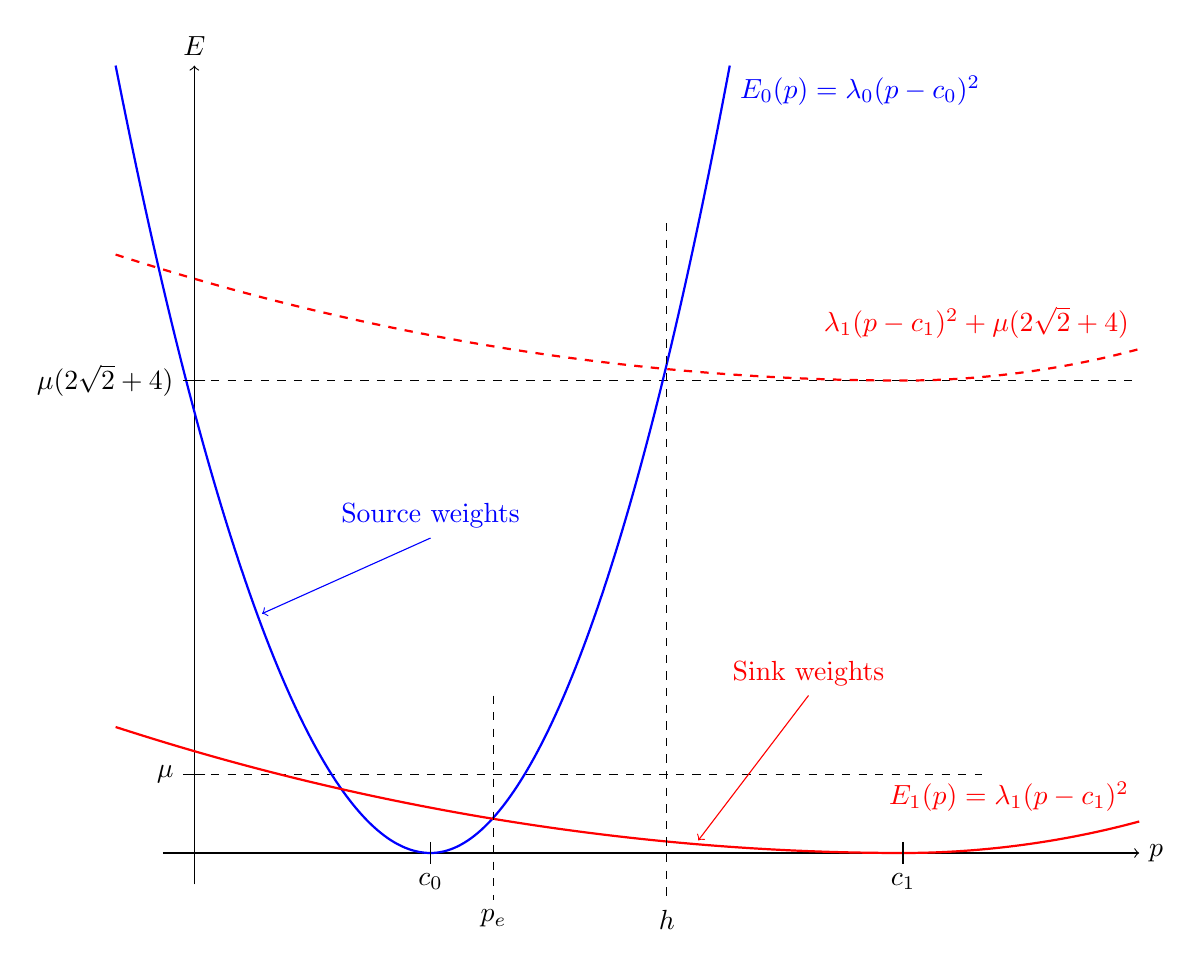
\begin{tikzpicture}[scale=2]
	\draw[->] (-0.2,0) -- (6,0) node[right] {$p$};
	\draw[->] (0,-0.2) -- (0,5) node[above] {$E$};
	
	\draw[dashed] (0,0.5) -- (5,0.5);
	\draw[dashed] (0,3) -- (6,3);
	\draw[blue,thick] (-0.5,5) parabola bend (1.5,0) (3.4,5) node[below right] {$E_0(p) = \lambda_0 (p-c_0)^2$};
	\draw[red,thick] (-0.5,0.8) parabola bend (4.5,0) (6,0.2) node[above left] {$E_1(p) = \lambda_1 (p-c_1)^2$};
	\draw[dashed,red,thick] (-0.5,3.8) parabola bend (4.5,3) (6,3.2) node[above left] {$\lambda_1 (p-c_1)^2 + \mu(2\sqrt{2}+4)$};
	\draw[shift={(1.5,0)}] (0pt,2pt) -- (0pt,-2pt) node[below] {$c_0$};
	\draw[shift={(4.5,0)}] (0pt,2pt) -- (0pt,-2pt) node[below] {$c_1$};
	\draw[shift={(0,0.5)}] (2pt,0pt) -- (-2pt,0pt) node[left] {$\mu$};
	\draw[shift={(0,3)}] (2pt,0pt) -- (-2pt,0pt) node[left] {$\mu(2\sqrt{2}+4)$};
	
	\draw[dashed,black] (3.0,4) -- (3.0,-0.3) node[below] {$h$};
	\draw[dashed,black] (1.9,1) -- (1.9,-0.3) node[below] {$p_e$};
	%\draw[dashed,black] (0.94,1) -- (0.94,-0.3) node[below] {$p_e$};
	
	\draw[blue,<-] (0.43,1.52) -- (1.5,2) node[above] {Source weights};
	\draw[red,<-] (3.2,0.08) -- (3.9,1) node[above] {Sink weights};
	\end{tikzpicture}
	\caption{Data energy functions plot.}
	\label{fig:dataenergyplot}
\end{figure}

\begin{definition}[Analysis of the relationship between $p_e$ and $\alpha$]
	From \Cref{eq:pe} we note that there is one tunable parameter, i.e. $\alpha$. We can see that $p_e$ and $\alpha$ are inversely related. This is expressed mathematically as
\begin{equation*}\begin{split}
		\text{if } \alpha=1, p_e=c_0+\frac{c_1-c_0}{1+\sqrt{1}} = \frac{c_0+c_1}{2} \hspace{30pt}&\text{(midpoint between $c_0$ and $c_1$)}\\
		\lim_{\alpha\to\infty}p_e = \lim_{\alpha\to\infty}c_0+\frac{c_1-c_0}{1+\sqrt{1}} = c_0\hspace{30pt} &\text{(maximum $\alpha$ yields lowerbound on $p_e$)}\\
		\lim_{\alpha\to0}p_e = \lim_{\alpha\to0}c_0+\frac{c_1-c_0}{1+\sqrt{0}} = c_1\hspace{30pt} &\text{(minimum $\alpha$ yields upperbound on $p_e$)}
	\end{split}\end{equation*}
\end{definition}
The relationship between $p_e$ and $\alpha$ is illustrated in \Cref{fig:alphaperelationship}.
\begin{figure}[!h]
	\centering
	\begin{tikzpicture}[scale=1]
	\draw[->] (0,0) -- (15,0) node[right] {$p$};
	\draw[shift={(3,0)}] (0pt,4pt) -- (0pt,-4pt) node[below] {$c_0$};
	\draw[shift={(12,0)}] (0pt,4pt) -- (0pt,-4pt) node[below] {$c_1$};
	\draw[dashed,black] (7.5,1.5) node[above] {$p_e = \frac{c_0+c_1}{2}$} -- (7.5,-0.3) node[below] {$\alpha=1$};
	\draw[black,->,thick] (7.5,0.5) -- (5.5,0.5) node[above] {increasing $\alpha$} -- (4.5,0.5);
	\draw[black,->,thick] (7.5,0.5) -- (9.5,0.5) node[above] {decreasing $\alpha$} -- (10.5,0.5);
	\end{tikzpicture}
	\caption{Relationship between $\alpha$ and $p_e$.}
	\label{fig:alphaperelationship}
\end{figure}

\begin{definition}[Figuring $\alpha$]
	If we are able to make good estimates on $p_e$, $c_0$ and $c_1$ for the final segmented image, then it is possible to calculate $\alpha$ as follows:
	\begin{equation*}\begin{split}
		p_e &= c_0 + \frac{c_1-c_0}{\sqrt{\alpha} + 1} \\
		1+\sqrt{\alpha} &= \frac{c_1-c_0}{p_e-c_0}
		%\alpha &= \left( \frac{c_1-c_0}{p_e-c_0}-1 \right)^2
	\end{split}\end{equation*}
	\begin{equation}
		\alpha = \left( \frac{c_1-c_0}{p_e-c_0}-1 \right)^2
		\label{eq:alphaapproximation}
	\end{equation}
\end{definition}

\begin{definition}[Lowerbound on $\mu$]
	When we found the point, $p_e$, where the energies are equal in \Cref{eq:pe}, we ignored the other solution as it was not within the range from $c_0$ to $c_1$. Let this point be $p_{e^*}$. If this point is positive and $0<p_{e^*}<c_0$ then we must ensure that at no point within this range that the source flow saturates all the outgoing edges. This force a limit on how low $\mu$ can be. This is only of significant concern when $\alpha>1$. We only need to concern ourselve with the point $p=0$ as this is the point where the difference $E^i(0)-E^i(1)$ is the largest. The lowerbound on $\mu$ can be obtained as follows
	\begin{equation*}\begin{split}
		E^i(0)|_{p_i=0} &< E^i(1)|_{p_i=0} + \mu \left( 2\sqrt{2} + 4\right) \\
		\lambda_0c_0^2 &< \lambda_1c_1^2 + \mu \left( 2\sqrt{2} + 4\right) \\
		\therefore \mu \left( 2\sqrt{2} + 4\right) &> \lambda_0c_0^2 - \lambda_1c_1^2\\
		\mu &> \frac{\lambda_0c_0^2 - \lambda_1c_1^2}{\left( 2\sqrt{2} + 4\right)}
	\end{split}\end{equation*} 
\end{definition}
Taking into account the relation in \Cref{eq:l0l1dependancy} this becomes
\begin{equation}
	\mu > \frac{\lambda_1(\alpha c_0^2-c_1^2)}{\left( 2\sqrt{2} + 4\right)}
	\label{eq:mulowerbound}
\end{equation}

\begin{definition}[Absolutely in the source set] From \Cref{eq:sourcesaturation} we can see that there is a point beyond which all nodes which correspond to pixel value higher than that point will be saturated and have excess flow which means that they will be in the source set. We will call this point the \textit{saturation point} and denote it by $h$. This is shown in \Cref{fig:dataenergyplot}. This point can be determined as follows:
\begin{equation*}\begin{split}
	\lambda_0(h-c_0)^2 &> \lambda_1(h-c_1)^2 + f_{max} \\
	\lambda_0(h-c_0)^2 - \lambda_1(h-c_1)^2 &> f_{max} \\
	(\lambda_0-\lambda_1)h^2 + (-2\lambda_0 c_0 + 2\lambda_1 c_1)h + (\lambda_0 c_0^2 - \lambda_1 c_1^2-f_{max}) &> 0
\end{split}\end{equation*}
The solutions to $h$ are
\begin{equation*}\begin{split}
	h = \frac{ (2\lambda_0 c_0 - 2\lambda_1 c_1) \pm \sqrt{(-2\lambda_0 c_0 + 2\lambda_1 c_1)^2-4(\lambda_0-\lambda_1)(\lambda_0 c_0^2 - \lambda_1 c_1^2-f_{max})}}{2(\lambda_0-\lambda_1)}
\end{split}\end{equation*}
Substituting the relation in \Cref{eq:l0l1dependancy}
\begin{equation*}\begin{split}
	h &= \frac{(\alpha c_0-c_1)\pm\sqrt{(c_1-\alpha c_0)^2-(\alpha-1)(\alpha c_0^2-c_1^2-\frac{f_{max}}{\lambda_1})}}{\alpha-1}\\
	&= \frac{(\alpha c_0-c_1)\pm\sqrt{\alpha(c_0-c_1)^2+\frac{f_{max}}{\lambda_1}(\alpha-1)}}{\alpha-1}
\end{split}\end{equation*}
If the $\mu$ is greater than the lowerbound in \Cref{eq:mulowerbound} then there is only one solution to $h$ which is of importance. This is the positive solution for $h$ which is
\begin{equation}
	h = \frac{(\alpha c_0-c_1)+\sqrt{\alpha(c_0-c_1)^2+\frac{\mu(2\sqrt{2}+4)}{\lambda_1}(\alpha-1)}}{\alpha-1}
\end{equation}
This point is marked off in \Cref{fig:dataenergyplot}.
\end{definition}

\begin{definition}[Determining $\lambda_1$] Given good approximations for $c_0$, $c_1$, $\alpha$, $h$ and $\mu$, we can calculate the appropriate value for $\lambda_1$. We proceed from \Cref{eq:sourcesaturation} as follows
\begin{equation*}\begin{split}
	\lambda_0(h-c_0)^2 &= \lambda_1(h-c_1)^2 + \mu(2\sqrt{2}+4)\\
	\lambda_1(\alpha(h-c_0)^2-(h-c_1)^2) &= \mu(2\sqrt{2}+4)
\end{split}\end{equation*}
\begin{equation}
	\lambda_1 = \frac{\mu(2\sqrt{2}+4)}{\alpha(h-c_0)^2-(h-c_1)^2}
	\label{eq:lambda1approximation}
\end{equation}
\end{definition}

The parameter estimation is based on the assumption that sufficiently good approximations for $c_0$, $c_1$, $p_e$ and $h$ can be obtained. From these approximation we calculate the approximation for $\alpha$ using \Cref{eq:alphaapproximation}. The parameters $\mu$ and $\alpha$ are related and aren't seperable, therefore we set choose to set $\mu$. We can then calculate $\lambda_1$ using \Cref{eq:lambda1approximation}. For the chosen $\mu$ we can calculate the upperbound on $\alpha$ to ensure that the constraint \Cref{eq:mulowerbound} is met. The constraint on $\lambda_1$ is calculated as follows
\begin{equation*}
\mu\left( 2\sqrt{2} + 4 \right) > \lambda_1(\alpha c_0^2 - c_1^2)
\end{equation*}
\begin{equation}
	\lambda_1 < \frac{\mu\left( 2\sqrt{2} + 4 \right)}{\alpha c_0^2 - c_1^2}
\end{equation}
Finally $\lambda_0$ can be calculated using \Cref{eq:l0l1dependancy}.

\subsection{Tuning Parameters for Fluorescence Microscopy}
\label{sec:cvgc_parameterestimation}

\textcolor{red}{What sort of image properties are we tuning for? E.g. dark bg, low contrast, etc. Parameters limits and ranges.}

\section{Experimental Results}
\label{sec:cvgc_experimentalresults}

\textcolor{red}{Present and analyse the experimental results.}
